\section{Sensitivity and robustness}

Fixed-parameter checks test local dependence; reselection repeats the candidate search and deployment rule. Permutation examines additional dimensions without aligned customer information.

\subsection{Named features and reduced geometry}

Fixed parameter deletion identifies category behaviour as the strongest local influence on the rich partitions. Removing distinct top categories reduces agreement with the full rich result to ARI 0.189 for CLASSIX and 0.516 for K Means. Removing top category share gives ARI 0.238 and 0.517. Every other CLASSIX deletion remains between 0.927 and 0.967. The corresponding K Means values remain between 0.855 and 0.991. Activity span and mean interevent time have the next largest effect on K Means, with ARI 0.874 and 0.855. Influence is unevenly distributed across the named variables, but category information alone does not generate a preferable segmentation.

The PCA diagnostic preserves 91.32 per cent of standardised rich variance in six components. It is a fixed-parameter local diagnostic rather than PCA-space model selection. K Means in this reduced space agrees with the named rich partition at ARI 0.995 and has silhouette 0.390 compared with 0.351. CLASSIX retains three clusters, lowers noise from 218 to 71 customers and agrees with the named result at ARI 0.920. Its silhouette is 0.304 compared with 0.291. Mean resampling ARI is 0.995 for reduced K Means and 0.987 for reduced CLASSIX. Much of the rich partition therefore survives dimension reduction, without proving that redundancy is irrelevant or six components optimal. Rotated components lose the direct meaning needed for named-feature explanations.

\begin{figure}[htbp]
\centering
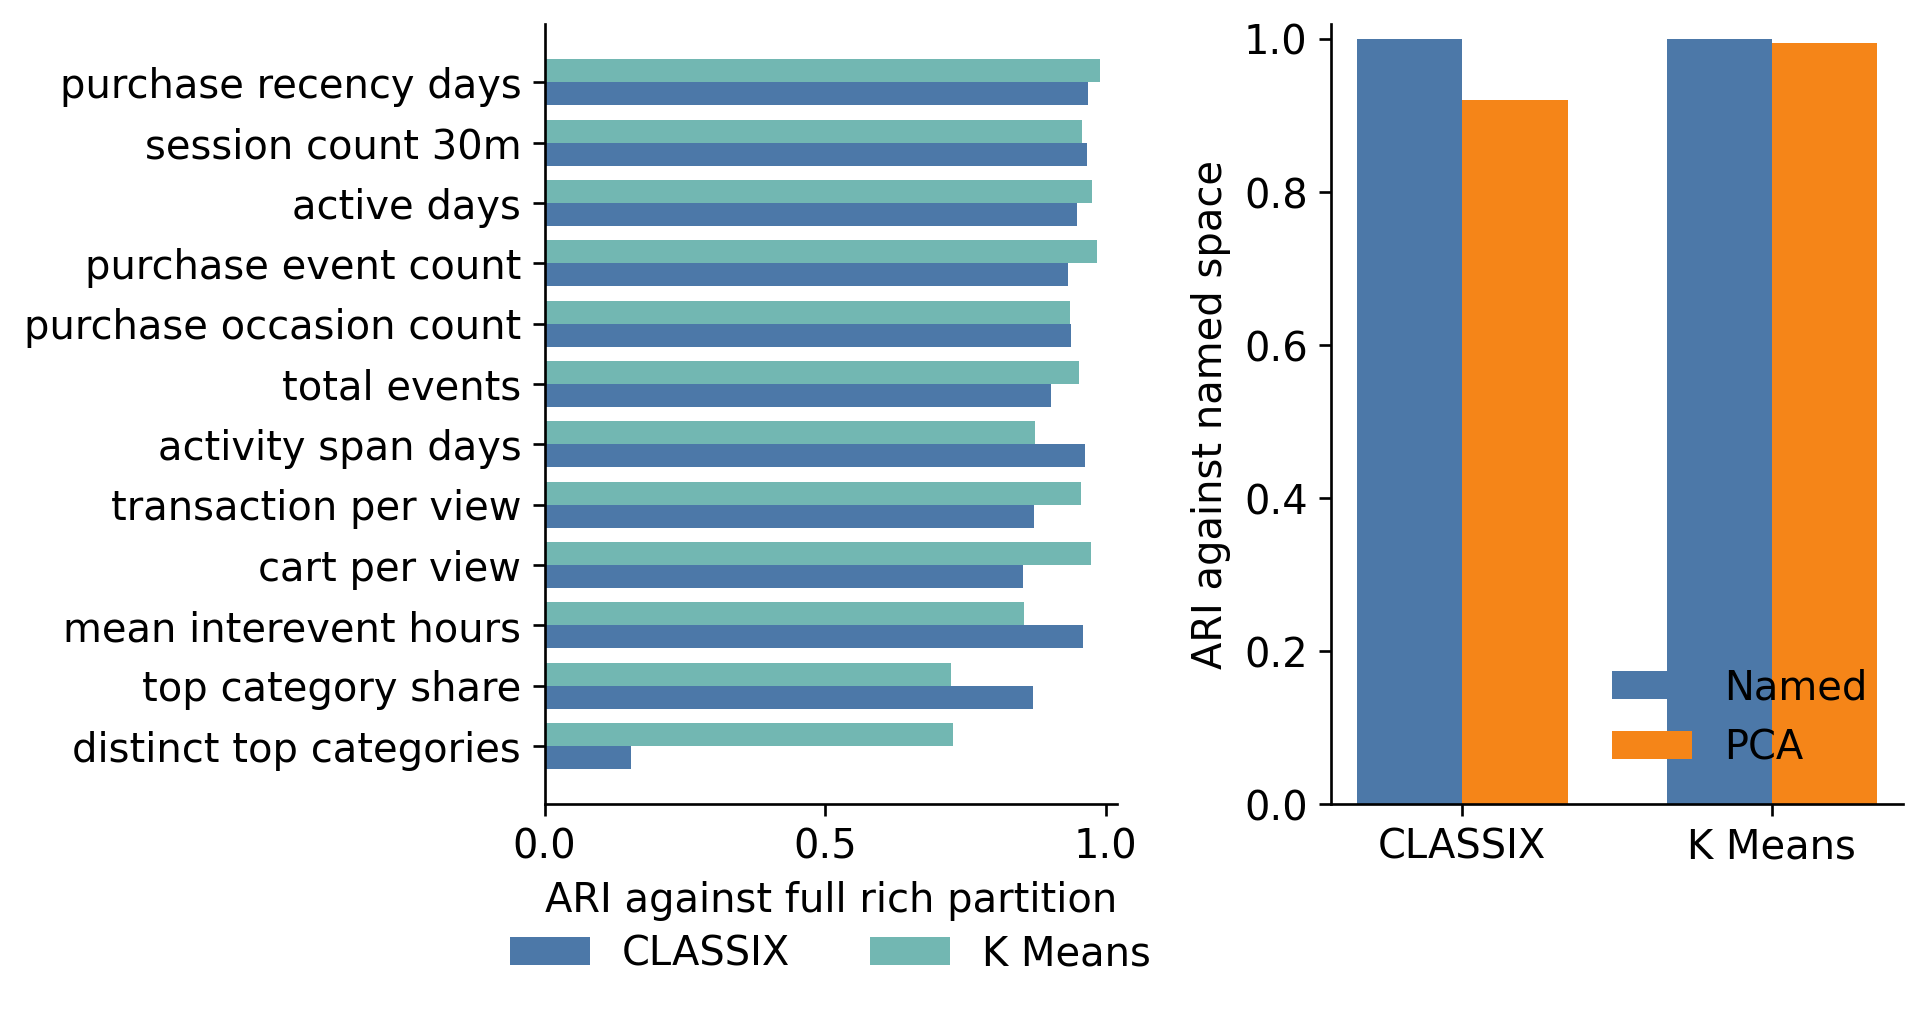
\includegraphics[width=0.80\textwidth]{figures/sensitivity_summary.png}
\caption{Reselected feature deletion and PCA diagnostics}
\label{fig:sensitivity_summary}
\end{figure}

Complete reselection confirms that category information creates the largest structural turn. All twenty two scenarios produce a deployment acceptable candidate. Removing distinct top categories changes CLASSIX to eleven clusters with ARI 0.153 against the full rich partition. K Means changes to two clusters with ARI 0.728. Removing the whole category block produces seven CLASSIX clusters with ARI 0.126 and two K Means clusters with ARI 0.729. The progressive endpoints reproduce the compact and rich primary partitions exactly. These 4,334 candidate fits show that the category effect persists when parameters and cluster counts are allowed to change.

CLASSIX sensitivity is distributed across the grid rather than concentrated at one radius. Deployment acceptable candidates occur at twenty three of thirty one compact radii from 0.35 to 1.45 and twenty rich radii from 0.30 to 1.25. Minimum size 1 produces no acceptable candidate in either representation. Minimum sizes 5 and 10 produce 23 and 32 acceptable compact candidates, compared with 19 and 27 rich candidates.

\subsection{Perturbation and temporal assumptions}
\label{sec:perturbation_results}

Small Gaussian perturbations leave the selected CLASSIX partitions almost unchanged. Compact agreement remains ARI 1 through a noise standard deviation of 0.001. At 0.01 the mean ARI is 0.999 and the minimum is 0.996. Rich agreement is also exact through 0.0001. It falls to a mean of 0.995 at 0.001 and 0.985 at 0.01, with minima of 0.985 and 0.962. Rich assignments are more sensitive at the tested scales, without wholesale reassignment. These trials cannot certify all nearby inputs. In particular, the rich fit uses density merging, outside the distance-only certificate of Section~\ref{sec:local_certificate}.

Reconstructing sessions from raw events gives a similar qualified result. The selected thirty minute window reproduces both partitions exactly. A fifteen minute window gives ARI 0.976 for K Means and 0.971 for CLASSIX. A sixty minute window gives ARI 0.985 and 0.959. The four cluster K Means result and the three cluster CLASSIX result persist at both alternative windows, although the CLASSIX noise count changes from 218 to 220 and 239. The conclusions do not arise solely from choosing exactly thirty minutes, while the detailed assignments still depend on the session convention.

\subsection{Dimensionality control}

The permutation control sets a stricter boundary on causal interpretation. The compact columns remain unchanged while the nine additional dimensions are independently permuted across customers. These columns preserve their marginal distributions but destroy their joint relationship with the compact representation and with each other. With the compact K Means setting held fixed, adding all nine permuted columns lowers agreement with the compact partition to ARI 0.017 and silhouette to 0.127. With the compact CLASSIX setting held fixed, adding even one permuted dimension produces a single cluster and ARI 0.

The single deterministic permutation control is an existence demonstration rather than a variance decomposition. Standardisation gives each added variable comparable weight, so random added dimensions can alter distances, principal directions and radius neighbourhoods in at least one realised order. The control does not estimate how much of the observed compact-to-rich difference is caused by dimensionality. Named feature deletion and PCA separately show that category and temporal information contribute reproducible structure in the observed rich representation.

\section{Integrated discussion and validity limits}

\paragraph{Strongly supported findings}
For both algorithms, representation materially changes assignments on the same purchasers, including under matched parameters. High within-space repeatability does not contradict between-space disagreement. Explanation also changes: rich CLASSIX has more aggregation groups, while ExKMC's relative fidelity reverses as its budget increases. The single passing rich K Means cluster demonstrates why geometry, repeatability, rule approximation and operational addressability require separate evidence.

\paragraph{Conditionally supported findings}
Deletion and reselection identify category dependence; PCA preserves much fitted structure, and tested numerical changes and session windows retain substantial agreement. These findings concern specific diagnostics, not all preprocessing choices. The permutation demonstrates a possible dimensionality effect without quantifying its causal share. Deployment cutoffs are operational choices; resampling holds selected parameters fixed; benchmark rankings need not transfer to purchasers. The local certificate requires unmeasured margins and excludes density merging.

\paragraph{Unresolved questions and evidence limits}
One anonymous purchaser log cannot establish general customer types. Category joins cover 76.16 per cent of events; 1,168 purchasers have no known category, and zero ratios can reflect absent recorded views. No demographic, price, revenue or response data justify labels such as valuable or loyal.

Neither intrinsic provenance nor agreement with a K Means predictor measures human comprehension. Addressability checks size, coverage and named-feature distinctiveness, not commercial outcomes. Prospective interventions and user evaluation would be needed to establish those benefits. The contribution is the joint examination of separate clustering and explanation properties under representation change, not universal superiority of richer features.
